% !TEX root=../main.tex

\section{Top and TopHat}
\label{sec:tophat}
This section briefly introduces the task-oriented programming paradigm \TOP,
followed by a description of the task-oriented programming language \TOPHAT.



\subsection{Top}

Task Oriented Programming (\TOP) is a reasonably new programming paradigm, first introduced by Plasmeijer et al.~\cite{DBLP:conf/ppdp/PlasmeijerLMAK12}.
It was invented in order to improve the way software that models collaboration is developed.
The aim of the paradigm is to provide programmers with a very high level of abstraction while still being expressive enough to describe real world collaboration.
Since the idea was introduced, a lot of research as been done on \TOP, but the basic principle has remained the same.
Programmers describe what work needs to be done in what way, by writing so-called tasks.
From the task specifications, the entire application is generated.

Tasks consist of the following components.

\subsubsection{Editors}

  These form the entry points for interaction and communication with the outside world.

  As mentioned, editors are the entry points for interaction and communication with the outside world.
  Editors are the most basic tasks.
  Editors are an abstraction over widgets in a \GUI library or on webpage forms.
  Users can change the value held by an editor, in the same way they can manipulate widgets in a \GUI.

  When a \TOP implementation generates an application from a task specification, it derives user interfaces for the editors.
  The appearance of an editor is influenced by its type.
  For example, an editor for a string can be represented by a simple input field, a date by a calendar, and a location by a pin on a map.

\subsubsection{Combinators}

  The order in which editors and tasks are executed is specified with combinators. Tasks can be performed in sequence, in parallel or a choice can be made between tasks.


  Editors can be combined into larger tasks using combinators.
  Combinators describe the way people collaborate.
  Tasks can be performed in sequence or in parallel, or there is a choice between two tasks.

\subsubsection{Shared data}

 Tasks communicate with each other by passing data along control flow, or via globally shared data stores.


% \TOP implementations like iTasks~\cite{????} also leverage aspects of the host language in order to allow for a higher level of abstraction,
% such as generic programming and higher order tasks. \todo{is dit wel of niet top?}
%
%
% The next section describes the formal \TOP implementation \TOPHAT.


\subsection{TopHat}

TopHat (\TOPHAT) implements \TOP by embedding the task language in a simply typed lambda calculus with references, conditionals, booleans, integers, strings, pairs, lists and unary and binary operations on these types.
References are used to model the shared data component of \TOP.
Below, the different components of \TOPHAT are explained in detail.
The complete syntax and semantics can be found in previous work~\cite{Steenvoorden2019}.


\subsubsection{Editors}

There are three different editors in \TOPHAT.
\begin{description}
  \item[$\Edit v$] Valued editor.\\
    This editor holds a value $v$ of a certain type.
    The user can replace the value by a new value of the same type.
  \item[$\Enter \tau$] Unvalued editor.\\
    This editor holds no value, and can receive a value of type $\tau$.
    When that happens, it turns into a valued editor.
  \item[$\Update l$] Shared editor.\\
    This editor refers to a store location $l$.
    Its observable value is the value stored at that location.
    When it receives a new value, this value will be stored at location $l$.
\end{description}


\subsubsection{Combinators}

The following combinators are available in \TOPHAT.
Here, $t$ stands for tasks and $e$ for arbitrary expressions.
The concrete syntax of the language is described in previous work~\cite{Steenvoorden2019}.
\begin{description}
  \item[$t \Then e$] Step.\\
    Users can work on task $t$.
    As soon as $t$ has a value, that value is passed on to the right hand side $e$.
    The expression $e$ is a function, taking the value as an argument, resulting in a new task.
  \item[$t \Next e$] User Step.\\
    Users can work on task $t$.
    When $t$ has a value, the step becomes enabled.
    Users can then send a continue event to the combinator.
    When that happens, the value of $t$ is passed to the right hand side, with which it continues.
  \item[$t_1 \And t_2$] Composition.\\
    Users can work on tasks $t_1$ and $t_2$ in parallel.
  \item[$t_1 \Or t_2$] Choice.\\
    The system chooses between $t_1$ or $t_2$,
    based on which task first has a value.
    If both tasks have a value, the system chooses the left one.
  \item[$e_1 \Xor e_2$] User choice.\\
    A user has to make a choice between either the left or the right hand side.
    The user continues to work on the chosen task.
\end{description}

In addition to editors and combinators, \TOPHAT also contains the fail task ($\Fail$).
Programmers can use this task to indicate that a task is not reachable or viable.
When the right hand side of a step combinator evaluates to $\Fail$, the step will not proceed to that task.



\subsubsection{Observations}

Several observations can be made on tasks.
Using the value function $\Value$, the current value of a task can be determined.
The value function is a partial function, since not all tasks have a value.
For example empty editors and steps do not have a value.

One can also observe whether or not a task is failing, by means of the failing function $\Failing$.
The task $\Fail$ is failing, as is a parallel combination of failing tasks ($\Fail \And \Fail$).

The step combinator makes use of both functions in order to determine if it can step.
First, it uses $\Value$ to see if the left hand side produces a value.
If that is the case, it uses the $\Failing$ function to see if it is safe to step to the right hand side.
The complete definition of the value and failing function are discussed in previous work~\cite{Steenvoorden2019}.

\usemacro{O-Value}

\subsubsection{Input}

Input events drive evaluation of tasks.
Because tasks are typed, input is typed as well.
Editors only accept input of the correct type.
Examples are replacing a value in an editor,
or sending a continue event to a user step.
When the system receives a valid event, it gives this event to the current task, which reduces to a new task.
Everything in between interaction steps is evaluated atomically with respect to inputs.
% In this way the system communicates with the environment.

Input events are synchronous, which means the order of execution is completely determined by the order of the events.
In particular, the order of input events determine the progression of parallel branches.

\fixme{Say something about the different semantics, since those will be used in a later section!}

\begin{figure}[h]
  \centering
  \includegraphics[width=\columnwidth,page=5]{figures/drawings-crop.pdf}
  \caption{
    Semantic functions defined in this report and their relation.
  }
  \label{fig:semantic-functions}
\end{figure}

\boxed{\RelationE}
\boxed{\RelationS}
\boxed{\RelationN}
\boxed{\RelationH}
\boxed{\RelationI}

\begin{figure}[ht]
  \small
  \usemacro{G-Values-Compact}
  \usemacro{G-Tasks-Compact}
  \caption{Syntax of values in \TOPHAT.}
  \label{fig:syntaxvalues}
\end{figure}
